% Five operational surfaces as one arc for Ch21 ("Measuring & Operating Agents") — the Vol 3 spine.
% Standalone TikZ; compiled by `book-scaffold build-figures` via pdflatex -> pdftocairo -> SVG.
% Left-to-right: measure (eval) -> see (observability) -> spend (cost) -> oversee (HITL) -> defend
% (security). A dashed return arrow loops failures back into the eval suite (the ch28 loop).
\documentclass[tikz,border=4mm]{standalone}
\usepackage{tikz}
\usetikzlibrary{positioning, arrows.meta, calc}

\begin{document}
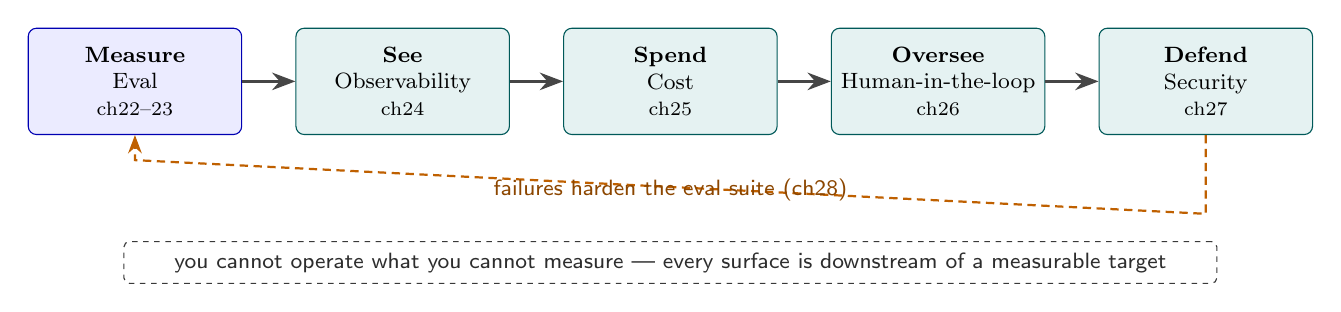
\begin{tikzpicture}[
  font=\sffamily,
  stage/.style={draw=teal!70!black, fill=teal!10, rounded corners=3pt, align=center,
    text width=2.5cm, minimum height=1.35cm, inner sep=3pt, font=\footnotesize},
  first/.style={draw=blue!70!black, fill=blue!8, rounded corners=3pt, align=center,
    text width=2.5cm, minimum height=1.35cm, inner sep=3pt, font=\footnotesize},
  flow/.style={-Stealth, very thick, draw=gray!55!black},
  loop/.style={-Stealth, thick, draw=orange!75!black, dash pattern=on 3pt off 2pt}
]

% five stages, left to right (eval first, highlighted as the target)
\node[first] (s1) at (0,0)    {\textbf{Measure}\\Eval\\{\scriptsize ch22--23}};
\node[stage] (s2) at (3.4,0)  {\textbf{See}\\Observability\\{\scriptsize ch24}};
\node[stage] (s3) at (6.8,0)  {\textbf{Spend}\\Cost\\{\scriptsize ch25}};
\node[stage] (s4) at (10.2,0) {\textbf{Oversee}\\Human-in-the-loop\\{\scriptsize ch26}};
\node[stage] (s5) at (13.6,0) {\textbf{Defend}\\Security\\{\scriptsize ch27}};

\draw[flow] (s1) -- (s2);
\draw[flow] (s2) -- (s3);
\draw[flow] (s3) -- (s4);
\draw[flow] (s4) -- (s5);

% dashed return arrow: failures harden the eval suite (the ch28 loop)
\draw[loop] (s5.south) -- ++(0,-1.0) -- (0,-1.0) -- (s1.south);
\node[font=\sffamily\footnotesize, text=orange!55!black] at (6.8,-1.38) {failures harden the eval suite (ch28)};

% caption strip beneath
\node[draw=gray!45!black, dash pattern=on 2pt off 2pt, rounded corners=2pt, align=center,
  text width=13.6cm, inner sep=4pt, font=\sffamily\footnotesize, text=gray!35!black]
  at (6.8,-2.3) {you cannot operate what you cannot measure --- every surface is downstream of a measurable target};

\end{tikzpicture}
\end{document}
